\documentclass[11pt]{article}
\usepackage[utf8]{inputenc}
\usepackage[dvips]{graphicx}
\usepackage{fancybox}
\usepackage{verbatim}
\usepackage{multirow,array}
\usepackage{latexsym}
\usepackage{alltt}
\usepackage{hyperref}
\usepackage{textcomp}
\usepackage{color}
\usepackage{amsmath}
\usepackage{amsfonts}
\usepackage{tikz}
\usepackage{float}
\usepackage[hmargin=3cm,vmargin=5.0cm]{geometry}
%\topmargin=0cm
\topmargin=-2cm
\addtolength{\textheight}{6.5cm}
\addtolength{\textwidth}{2.0cm}
%\setlength{\leftmargin}{-5cm}
\setlength{\oddsidemargin}{0.0cm}
\setlength{\evensidemargin}{0.0cm}

\newcommand{\tikzmark}[1]{\tikz[overlay, remember picture] \coordinate (#1);}
\begin{document}

\section*{Student Information } 
%Write your full name and id number between the colon and newline
%Put one empty space character after colon and before newline
Full Name : mergen \\

% Write your answers below the section tags

\section*{Answer 1}
\subsection*{a)}
\begin{figure}[H]
	\centering
	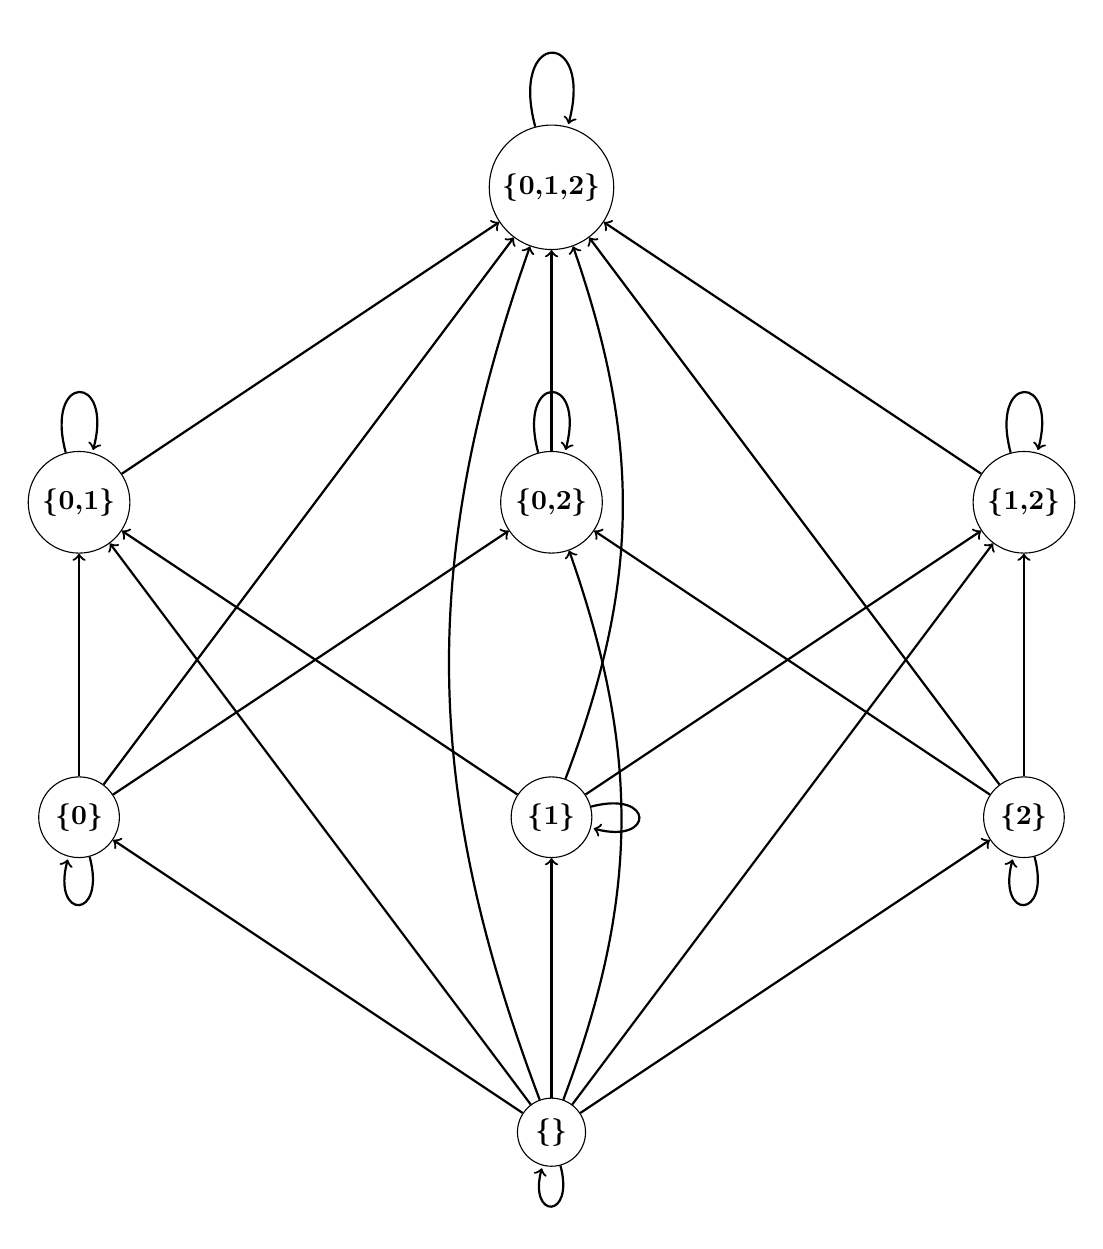
\begin{tikzpicture}
	\node[shape=circle,draw=black] (a) at (6, 12)     {\textbf{\{0,1,2\}}};
	
	\node[shape=circle,draw=black] (b) at (0, 8)      {\textbf{\{0,1\}}};
	\node[shape=circle,draw=black] (c) at (6, 8)      {\textbf{\{0,2\}}};
	\node[shape=circle,draw=black] (d) at (12, 8)      {\textbf{\{1,2\}}};
	
	\node[shape=circle,draw=black] (e) at (0, 4)      {\textbf{\{0\}}};
	\node[shape=circle,draw=black] (f) at (6, 4)      {\textbf{\{1\}}};
	\node[shape=circle,draw=black] (g) at (12, 4)      {\textbf{\{2\}}};
	
	\node[shape=circle,draw=black] (j) at (6, 0)      {\textbf{\{\empty\}}};
	
	
    \path[->, thick] (a) edge [loop above] (a);
    \path[->, thick] (b) edge [loop above] (b);
    \path[->, thick] (c) edge [loop above] (c);
    \path[->, thick] (d) edge [loop above] (d);
    \path[->, thick] (e) edge [loop below] (e);
    \path[->, thick] (f) edge [loop right] (f);
    \path[->, thick] (g) edge [loop below] (g);
    \path[->, thick] (j) edge [loop below] (j);

    

    \path[->, thick] (e) edge (b);
    \path[->, thick] (e) edge (c);
    \path[->, thick] (e) edge (a);

    \path[->, thick] (b) edge (a);
    \path[->, thick] (c) edge (a);

    \path[->, thick] (d) edge (a);
    
    \path[->, thick] (f) edge (b);
    \path[->, thick] (f) edge (d);
    \path[->, thick] (f) edge [bend right=20] (a);
    
    \path[->, thick] (g) edge (a);
    \path[->, thick] (g) edge (c);
    \path[->, thick] (g) edge (d);
    
    \path[->, thick] (j) edge [bend left=20] (a);
    \path[->, thick] (j) edge (b);
    \path[->, thick] (j) edge [bend right=20]  (c);
    \path[->, thick] (j) edge (d);
    \path[->, thick] (j) edge (e);
    \path[->, thick] (j) edge (f);
    \path[->, thick] (j) edge (g);
    
    
    
    
    
    
	\end{tikzpicture} 
	\caption{R in Q1, as a directed graph.}	
	\label{rdg1}
\end{figure}

\subsection*{b)}
\text{Proving that \textbf{(S,R)} is a poset requires 3 properties of partial ordering sets to be acquired: reflexivity,}\\
\text{anti-symmetry and transitivity.}\\
\text{From now on we use the definition of \textbf{R} and \textbf{S}:}\\
(1)\[S = \{w|w\in P(\{0,1,2\})\}\]\\
(2)\[R = \{(w_{1},w_{2})|w_{1}\in S,w_{2}\in S,w_{1} \subseteq w_{2}\}\]\\
\begin{itemize}
    \item reflexivity: As we know each set is a subset of itself(every element on the directed graph has a loop bending to itself), we can simply say the graph is reflexive.
    \item Since there are no two edges between two vertices with different directions, the graph is anti-symmetric.
    \item From the graph we can see that does not matter which path taken, it is possible to go \{0,1,2\} from \{\} that is; $\forall$w$_{1}$ $\forall$w$_{2}$ $\forall$w$_{3}$ $\in$S((w$_{1}$Rw$_{2}$ $\wedge$ w$_{2}$Rw$_{3}$) $\rightarrow$ w$_{1}$Rw$_{3}$). Therefore, from the definition of transitivity the graph is transitive.
    \item Since we have shown that the Graph 1 is reflexive, anti-symmetric, and transitive, the partial ordering (S,R) is a poset.
\end{itemize}
\subsection*{c)}
\begin{itemize}
    \item  \textbf{Definition 3, pg.651}
    \begin{quote}
        If $(S, \propto) $ is a poset and every two elements of $S$ are comparable, $S$ is called a totally ordered set, and $\propto$ is called a total order.
    \end{quote}
    \item $(S,R)$ is a poset, but since not each member of $S$ is comparable, $S$ is not a totally ordered set. That is, for example \{1,2\} $\subseteq$ \{1,2,3\} but \{1,2,3\} $\not\subseteq$ \{1,2\}.
\end{itemize}
\subsection*{d)}
\begin{figure}[H]
	\centering
	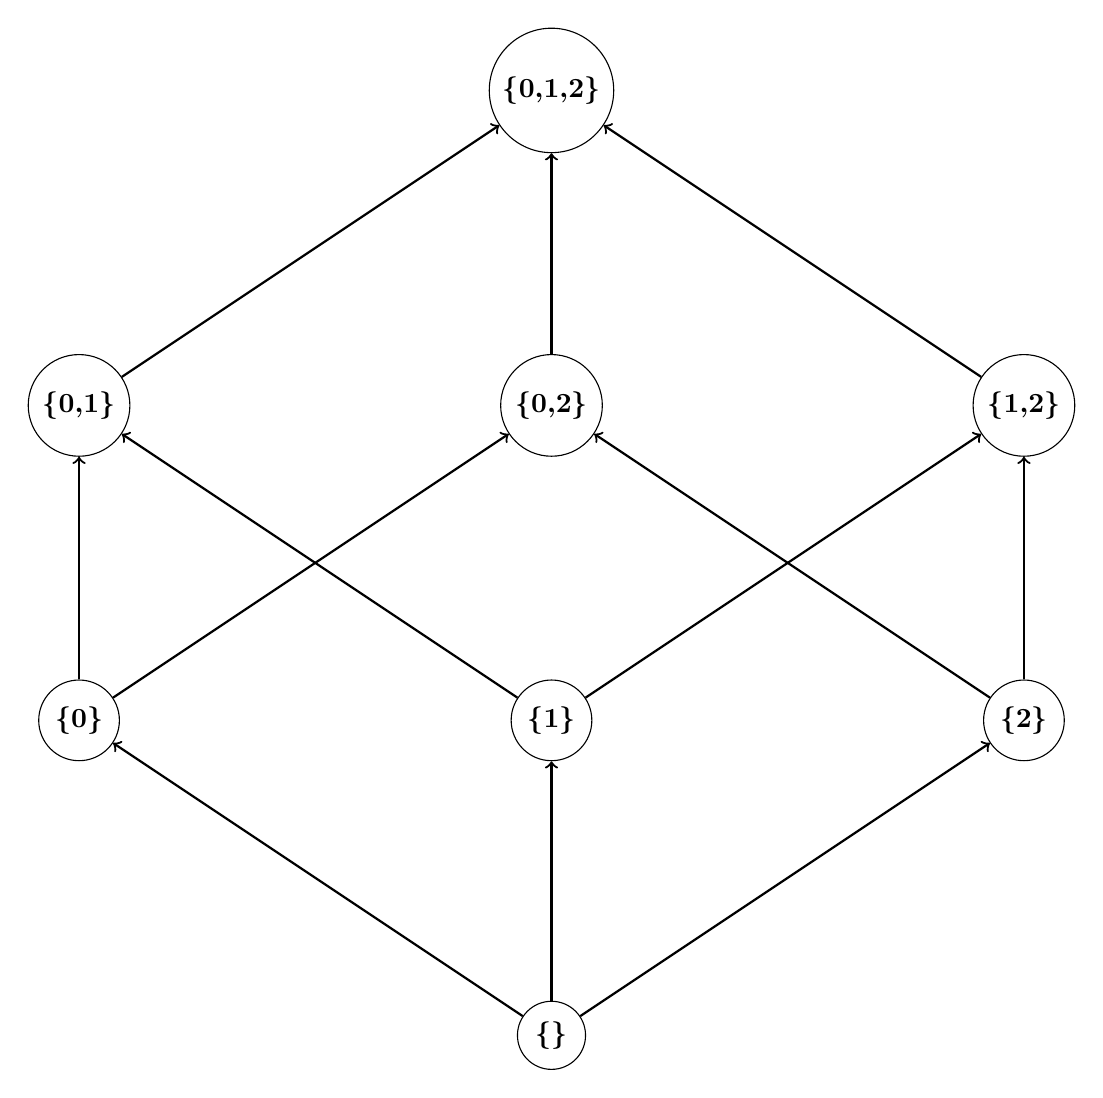
\begin{tikzpicture}
	\node[shape=circle,draw=black] (a) at (6, 12)     {\textbf{\{0,1,2\}}};
	
	\node[shape=circle,draw=black] (b) at (0, 8)      {\textbf{\{0,1\}}};
	\node[shape=circle,draw=black] (c) at (6, 8)      {\textbf{\{0,2\}}};
	\node[shape=circle,draw=black] (d) at (12, 8)      {\textbf{\{1,2\}}};
	
	\node[shape=circle,draw=black] (e) at (0, 4)      {\textbf{\{0\}}};
	\node[shape=circle,draw=black] (f) at (6, 4)      {\textbf{\{1\}}};
	\node[shape=circle,draw=black] (g) at (12, 4)      {\textbf{\{2\}}};
	
	\node[shape=circle,draw=black] (j) at (6, 0)      {\textbf{\{\empty\}}};
	

    \path[->, thick] (e) edge (b);
    \path[->, thick] (e) edge (c);

    \path[->, thick] (b) edge (a);
    \path[->, thick] (c) edge (a);

    \path[->, thick] (d) edge (a);
    
    \path[->, thick] (f) edge (b);
    \path[->, thick] (f) edge (d);
    
    \path[->, thick] (g) edge (c);
    \path[->, thick] (g) edge (d);
    
    \path[->, thick] (j) edge (e);
    \path[->, thick] (j) edge (f);
    \path[->, thick] (j) edge (g);
    
    
    
    
    
    
	\end{tikzpicture} 
	\caption{The Hasse-Diagram of (P(\{0,1,2\}),$\subseteq$)}	
	\label{rdg1}
\end{figure}
\textbf{Maximal element is }\{0,1,2\}\\
\textbf{Minimal element is }\{\}\\
\subsection*{e)}
\begin{itemize}
    \item The Lattice definition from the Section 9.6 of the textbook says that 
    \begin{quote}
        A partially ordered set in which every pair of elements has both a least upper bound and a greatest lower bound is called a lattice.
    \end{quote}
    \item As each two elements w$_{1}$ and w$_{2}$ in S, the least upper bound is as follows w$_{1}$ $\cup$ w$_{2}$
and the greatest lower bound is as follows w$_{1}$ $\cap$ w$_{2}$.
    \item Therefore,  (P(\{0,1,2\}),$\subseteq$) \textbf{constitutes a lattice}.
\end{itemize}
\section*{Answer 2}
\subsection*{a)}
\begin{table}[H]
\small
\centering
\caption{Adjacency list for directed graph G}  
\label{table:2}
\begin{tabular}{|c|c|}	%% specify column number and vertical lines
\hline 							%% line draw
\textbf{Initial Vertex} & \textbf{Terminal Vertex} \\
\hline
\hline
a &  \\	
b & a,c\\
c & f \\
d & a,c,d,e,g\\
e &  c,f,g\\
f &  b\\
f & d \\
\hline 

\end{tabular}
\end{table}
\subsection*{b)}
\[
   A_G = \qquad \bordermatrix{~  & \tikzmark{harrowleft} a & b & c & d & e & f & g \tikzmark{harrowright}  \cr
                     \tikzmark{varrowtop}
                     a & 0 & 0 & 0 & 0 & 0 & 0 & 0\cr
                     b & 1 & 0 & 1 & 0 & 0 & 0 & 0\cr
                     c & 0 & 0 & 0 & 0 & 0 & 1 & 0\cr
                     d & 1 & 0 & 1 & 1 & 1 & 0 & 1\cr
                     e & 0 & 0 & 1 & 0 & 0 & 1 & 1\cr
                     f & 0 & 1 & 0 & 0 & 0 & 0 & 0\cr
                     \tikzmark{varrowbottom}
                     g & 0 & 0 & 0 & 1 & 0 & 0 & 0\cr
                     }
\]
\subsection*{c)}
\text{deg$^{-}$(a) = 2, deg$^{+}$(a) = 0}\\
\text{deg$^{-}$(b) = 1, deg$^{+}$(b) = 2}\\
\text{deg$^{-}$(c) = 3, deg$^{+}$(c) = 1}\\
\text{deg$^{-}$(d) = 2, deg$^{+}$(d) = 5}\\
\text{deg$^{-}$(e) = 1, deg$^{+}$(e) = 3}\\
\text{deg$^{-}$(f) = 2, deg$^{+}$(f) = 1}\\
\text{deg$^{-}$(g) = 2, deg$^{+}$(g) = 1}\\

\begin{table}[H]
    \centering
    \begin{tabular}{|c|c|c|}	
    \hline 							
    & \textbf{In-degrees Count} & \textbf{Out-degrees Count}  \\
    \hline 
    \hline 
    a & 2 & 0 \\ \hline
    b & 1 & 2 \\ \hline
    c & 3 & 1 \\ \hline
    d & 2 & 5 \\ \hline
    e & 1 & 3 \\ \hline
    f & 2 & 1 \\ \hline
    g & 2 & 1 \\ \hline
    \end{tabular}
    \caption{ In-degrees and Out-degrees of every vertex of Graph G in Q2 }
    \end{table}
    
\subsection*{d)}
\begin{itemize}
    \item $d \rightarrow e \rightarrow f \rightarrow b \rightarrow a$
    \item $d \rightarrow c \rightarrow f \rightarrow b \rightarrow a$
    \item $e \rightarrow g \rightarrow d \rightarrow c \rightarrow f$
    \item $e \rightarrow c \rightarrow f \rightarrow b \rightarrow a$
    \item $g \rightarrow d \rightarrow c \rightarrow f \rightarrow b$
    \item $g \rightarrow d \rightarrow e \rightarrow c \rightarrow f$
\end{itemize}
\subsection*{e)}
\begin{itemize}
    \item $c \rightarrow f \rightarrow b \rightarrow c$
    \item $f \rightarrow b \rightarrow c \rightarrow f$
    \item $b \rightarrow c \rightarrow f \rightarrow b$
    \item $d \rightarrow e \rightarrow g \rightarrow d$
    \item $g \rightarrow d \rightarrow e \rightarrow g$
    \item $e \rightarrow g \rightarrow d \rightarrow e$
\end{itemize}
\subsection*{f)}
\begin{itemize}
    \item Since there is not a path from $a$ to $d$, we can say that the graph is \textbf{not} strongly connected.
    \item If we draw the \textbf{undirected graph} of the Graph G in Q2, we get the following;
\begin{figure}[H]
	\centering
	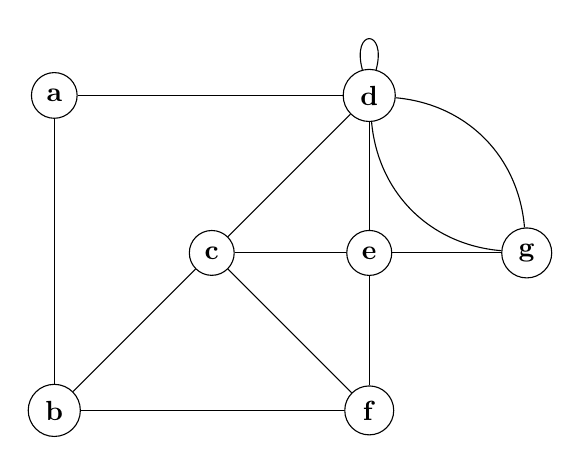
\begin{tikzpicture}[every loop/.style={}]
	\node[shape=circle,draw=black] (a) at (0, 4)     {\textbf{a}};
	\node[shape=circle,draw=black] (b) at (0, 0)     {\textbf{b}};
	\node[shape=circle,draw=black] (c) at (2, 2)     {\textbf{c}};
	\node[shape=circle,draw=black] (d) at (4, 4)     {\textbf{d}};
	\node[shape=circle,draw=black] (e) at (4, 2)     {\textbf{e}};
	\node[shape=circle,draw=black] (f) at (4, 0)     {\textbf{f}};
	\node[shape=circle,draw=black] (g) at (6, 2)     {\textbf{g}};
    \path[-] (a) edge (d);
    \path[-] (d) edge (d);
    \path[-] (d) edge  [bend left=40] (g);
    \path[-] (g) edge [bend left=40] (d);
    \path[-] (d) edge (e);
    \path[-] (e) edge (f);
    \path[-] (a) edge (d);
    \path[-] (c) edge (e);
    \path[-] (d) edge (c);
    \path[-] (e) edge (g);
    \path[-] (f) edge (c);
    \path[-] (f) edge (b);
    \path[-] (b) edge (c);
    \path[-] (b) edge (a);
    \path[every node/.style={font=\sffamily\small}]
        (d)   edge[loop above] (d);
	\end{tikzpicture} 
	\caption{The Undirected Graph of Graph G in Q2.}	
	\label{g2}
\end{figure}
    \item Since all vertices are connected to at least one other vertex, we can create paths between any given two vertices. % (Since the sub-graphs $(a, b, d)$, $(e,b,f)$, $(d,c,b)$, and $(b,c,g,f)$ are all complete loops).
    \item Since there is a path between every two vertices in the above undirected graph, we say 
    Graph \textit{G} is \textbf{weakly-connected.} (Definition 5, pg.721)
\end{itemize}
\subsection*{g)}
The strongly-connected components of $G$ are as follows;
\begin{itemize}
    \item the vertex $a$
    \item the subgraph consisting of the vertices $b,c,f$ and edges $(b,c),(c,f), and$ $(f,b)$
    \item the subgraph consisting of the vertices $d,e,g$ and edges $(d,e),(e,g), and$ $(g,d)$
\end{itemize}
\subsection*{h)}
\begin{figure}[H]
	\centering
	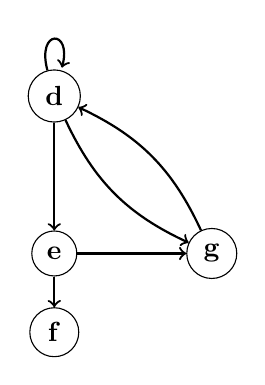
\begin{tikzpicture}
	
	\node[shape=circle,draw=black] (d) at (3, 3)     {\textbf{d}};
	\node[shape=circle,draw=black] (e) at (3, 1)     {\textbf{e}};
	\node[shape=circle,draw=black] (f) at (3, 0)     {\textbf{f}};
	\node[shape=circle,draw=black] (g) at (5, 1)     {\textbf{g}};

	\path[->, thick] (d) edge [loop above] (d);
	\path[->, thick] (d) edge (e);
	\path[->, thick] (d) edge [bend right=20] (g);
	\path[->, thick] (e) edge (f);
	\path[->, thick] (e) edge (g);
	\path[->, thick] (g) edge [bend right=20] (d);
	
	\end{tikzpicture} 
	\caption{Subgraph \textit{H} of \textit{G} induced by the vertices \{d, e, f, g\} $\subset$ V}	
	\label{g2}
\end{figure}


\[
   A_H = \qquad \bordermatrix{~  & \tikzmark{harrowleft} d & e & f & g \tikzmark{harrowright}  \cr
                     \tikzmark{varrowtop} d & 1 & 1 & 0 & 1 \cr
                     e & 0 & 0 & 1 & 1 \cr
                     f & 0 & 0 & 0 & 0 \cr
                     \tikzmark{varrowbottom}g & 1 & 0 & 0 & 0 \cr
                     }
\]

\text{From the Theorem(pg.723), number of different paths of length 3 from d to g in the subgraph \textit{H} will be}\\
\text{given by the value of A$^{3}_H$'s a$_{1,4}$ element.}\\

\[
   A^{3}_H = \qquad \bordermatrix{~  & \tikzmark{harrowleft} d & e & f & g \tikzmark{harrowright}  \cr
                     \tikzmark{varrowtop} d & 4 & 2 & 1 & 3 \cr
                     e & 1 & 1 & 0 & 1 \cr
                     f & 0 & 0 & 0 & 0 \cr
                     \tikzmark{varrowbottom}g & 2 & 1 & 1 & 2 \cr
                     }
\]
\text{Since a$_{1,4}$ = 3, there exist 3 different paths from d to g of length 3 in the subgraph \textit{H}.}\\
\section*{Answer 3}
\begin{table}[H]
    \centering
    \renewcommand{\arraystretch}{1.25}
    \begin{tabular}{|l||c|c|c|c|c|c|c|c|}	
    \hline 							
    \textbf{Vertex} & a & b & c & d & e & f & g & h \\ \hline
    \textbf{Degree} & 2 & 3 & 2 & 5 & 4 & 2 & 2 & 2  \\ \hline
    \end{tabular}
    \caption{ Degrees of each Vertex in Graph G in Q3 }
    \label{tq3}
    \end{table}

\subsection*{a}
\begin{itemize}
    \item  \textbf{Theorem 2} from the Section 10.5 of the textbook says that 
    \begin{quote}
        A connected multigraph has an Euler path but not an Euler circuit if and only if it has exactly two vertices of odd degree.
    \end{quote}
    \item Since the \textit{Graph G} is a connected multigraph, to check if the given graph has an Euler Path, we can simply check the degree of each vertex. On a graph with $n$ vertices, if $n-2$ vertices have even degree, and if the remaining 2 vertices have odd degrees, the given graph has an \textbf{Euler Path}. 
    \item When we look at Table \ref{tq3}, we can clearly see that not all vertices are of even degree, 2 vetices have odd degrees. 
    \item Therefore, \textit{Graph G} have an \textbf{Euler Path}.
    \item An example \textbf{Euler Path}: $ b \rightarrow a \rightarrow d \rightarrow b \rightarrow c \rightarrow d \rightarrow e \rightarrow f \rightarrow g \rightarrow h \rightarrow e \rightarrow d$
\end{itemize}

\subsection*{b}
\begin{itemize}
    \item  \textbf{Theorem 1} from the Section 10.5 of the textbook says that 
    \begin{quote}
        A connected multigraph with at least two vertices has an Euler circuit if and only if each of its vertices has even degree.
    \end{quote}
    \item Since the \textit{Graph G} is a connected multigraph with 8 vertices, to check if the given graph has an Euler Path, we can simply check the degree of each vertex. If all vertices have even degree, the given graph has an \textbf{Euler Circuit}. 
    \item When we look at Table \ref{tq3}, we can clearly see that not all vertices are of even degree. 
    \item Therefore, \textit{Graph G}does not have an \textbf{Euler Circuit}. 
    
\end{itemize}

\subsection*{c}

\begin{itemize}
    \item  \textbf{Definition 2} from the Section 10.5 of the textbook says that 
    \begin{quote}
        A simple path in a \textit{Graph G} that passes through every vertex exactly once is called a \textit{Hamilton Path}.
    \end{quote}
    
    \item By picking the following simple route, we can create a \textit{Hamilton Path};
    \subitem $ c \rightarrow b \rightarrow a \rightarrow d \rightarrow e \rightarrow h \rightarrow g \rightarrow f $
    \item Since we  were able to create a \textit{Hamilton Path}, we can say that \textit{Graph G} has a \textbf{Hamilton Path}. 
\end{itemize}

\subsection*{d}
\begin{itemize}
    \item  \textbf{Theorem 4 (Ore's Theorem)} from the Section 10.5 of the textbook says that 
    \begin{quote}
        If $G$ is a simple graph with $n$ vertices with $n \geq 3$ such that
$deg(u) + deg(v) \geq n$ for every pair of nonadjacent vertices $u$ and $v$ in $G$, then $G$ has a \textit{Hamilton Circuit}.
    \end{quote}
    \item Since the \textit{Graph G} is a simple graph with 8 vertices, if we find a pair of nonadjacent vertices with summed degrees less than 8, we can say that the given graph does not have a \textbf{Hamilton Circuit}. 
    \item Let us pick the nonadjacent vertices $b$ and $g$. When we look at Table \ref{tq3}, we can see that their degrees are 3 and 2, respectively. 
    \item We can easily see that $deg(b) + deg(g) \geq 8$ does not hold, and therefore  \textit{Graph G} does not have a \textbf{Hamilton Circuit}. 
\end{itemize}

\section*{Answer 4}
\text{Both \textbf{G} and \textbf{G'} have five vertices and five edges. Both have five vertices of degree two. Because \textbf{G} and}\\
\text{\textbf{G'} agree with respect to these invariants, it is reasonable to try to find an isomorphism \textit{f}. The function}\\
\text{\textit{f} with \textit{f(a) = a'}, \textit{ f(b) = e'}, \textit{ f(c) = d'}, \textit{ f(d) = c'}, \textit{ f(e) = b'} is a one-to-one correspondence between \textbf{G}}\\
\text{and \textbf{G'}. To see that correspondence preserves adjacency, note that adjacent vertices in \textbf{G} are a and b,}\\
\text{a and e, b and c, c and d, and d and e, and each of the pairs \textit{f(a) = a'} and \textit{ f(b) = e'}, \textit{ f(a) = a'} and}\\
\text{\textit{ f(e) = b'}, \textit{ f(b) = e'} and \textit{ f(c) = d'}, \textit{f(c) = d'} and \textit{ f(d) = c'}, and \textit{f(d) = c'} and \textit{ f(e) = b'} consists of}\\
\text{two adjacent vertices in \textit{G'}; with such adjacency matrices A$_G$ and A$_{G'}$ respectively. To see whether \textit{f}}\\
\text{preserves edges, we examine the adjacency matrix of \textbf{G},}\\




\[
   A_G = \qquad \bordermatrix{~  & \tikzmark{harrowleft} a & b & c & d & e\tikzmark{harrowright}  \cr
                     \tikzmark{varrowtop} a & 0 & 1 & 0 & 0 & 1 \cr
                     b & 1 & 0 & 1 & 0 & 0 \cr
                     c & 0 & 1 & 0 & 1 & 0 \cr
                     d & 0 & 0 & 1 & 0 & 1 \cr
                     \tikzmark{varrowbottom}e & 1 & 0 & 0 & 1 & 0 \cr
                     }
\]
\text{and the adjacency matrix of \textbf{G'} with the rows and columns labeled by the images of the correspond-}\\
\text{ing vertices in \textbf{G},}\\
\[
   A_{G'} = \qquad \bordermatrix{~  & \tikzmark{harrowleft} a' & e' & d' & c' & b'\tikzmark{harrowright}  \cr
                     \tikzmark{varrowtop} a' & 0 & 1 & 0 & 0 & 1 \cr
                     e' & 1 & 0 & 1 & 0 & 0 \cr
                     d' & 0 & 1 & 0 & 1 & 0 \cr
                     c' & 0 & 0 & 1 & 0 & 1 \cr
                     \tikzmark{varrowbottom}b' & 1 & 0 & 0 & 1 & 0 \cr
                     }
\]
\text{Because A$_G$ = A$_{G'}$, it follows that \textit{f} preserves edges. We conclude that \textit{f} is an 'isomorphism', so \textbf{G}}\\
\text{and \textbf{G'} are isomorphic.}\\
\section*{Answer 5}
\subsection*{a)}
\subsubsection*{Step 0}
\text{For this question, I used superscripts in the nodes as shortest distances from the starting node, namely $a$, }\\
for this graph\\
\begin{figure}[H]
	\centering
	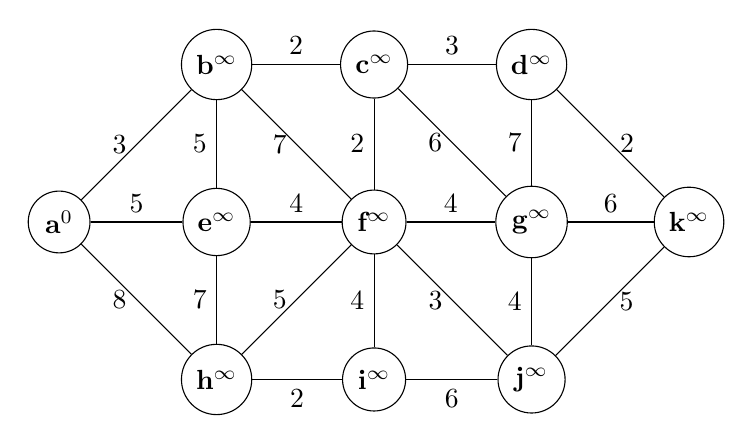
\begin{tikzpicture}
	\node[shape=circle,draw=black] (a) at (0, 2)     {\textbf{a$^0$}};
	\node[shape=circle,draw=black] (b) at (2, 4)     {\textbf{b$^\infty$}};
	\node[shape=circle,draw=black] (c) at (4, 4)     {\textbf{c$^\infty$}};
	\node[shape=circle,draw=black] (d) at (6, 4)     {\textbf{d$^\infty$}};
	\node[shape=circle,draw=black] (e) at (2, 2)     {\textbf{e$^\infty$}};
	\node[shape=circle,draw=black] (f) at (4, 2)     {\textbf{f$^\infty$}};
	\node[shape=circle,draw=black] (g) at (6, 2)     {\textbf{g$^\infty$}};
	\node[shape=circle,draw=black] (h) at (2, 0)     {\textbf{h$^\infty$}};
	\node[shape=circle,draw=black] (i) at (4, 0)     {\textbf{i$^\infty$}};
	\node[shape=circle,draw=black] (j) at (6, 0)     {\textbf{j$^\infty$}};;
	\node[shape=circle,draw=black] (k) at (8, 2)     {\textbf{k$^\infty$}};

	\path[-] (a) edge node[left]{3} (b);
	\path[-] (a) edge node[above]{5} (e);
	\path[-] (a) edge node[left]{8} (h);
	\path[-] (b) edge node[left]{5} (e);
	\path[-] (b) edge node[left]{7} (f);
	\path[-] (b) edge node[above]{2} (c);
	\path[-] (e) edge node[above]{4} (f);
	\path[-] (e) edge node[left]{7} (h);
	\path[-] (h) edge node[left]{5} (f);	
	\path[-] (h) edge node[below]{2} (i);	
	\path[-] (c) edge node[above]{3} (d);
	\path[-] (c) edge node[left]{6} (g);
	\path[-] (c) edge node[left]{2} (f);
	\path[-] (f) edge node[above]{4} (g);
	\path[-] (f) edge node[left]{3} (j);
	\path[-] (f) edge node[left]{4} (i);
	\path[-] (i) edge node[below]{6} (j);	
	\path[-] (d) edge node[right]{2} (k);
	\path[-] (d) edge node[left]{7} (g);
	\path[-] (g) edge node[above]{6} (k);
	\path[-] (g) edge node[left]{4} (j);
	\path[-] (j) edge node[right]{5} (k);
		
	\end{tikzpicture} 
	\caption{Initial conditions}
	\label{gg0}
\end{figure}

\subsubsection*{Step 1}
By visiting the \textit{unvisited} neighbouring nodes of $a$, we get the following graph.
\begin{figure}[H]
	\centering
	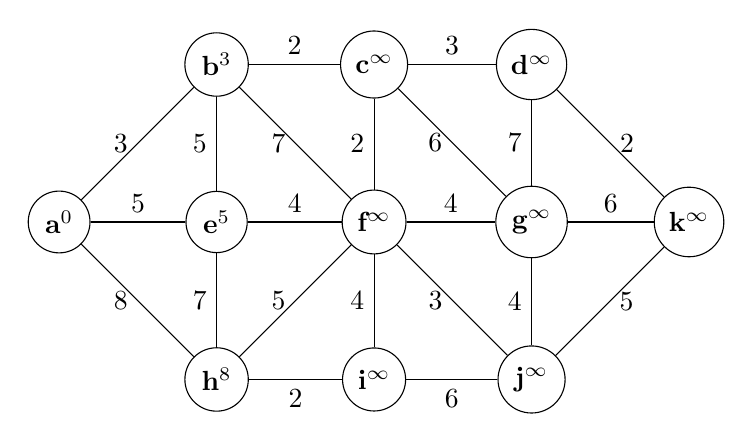
\begin{tikzpicture}
	\node[shape=circle,draw=black] (a) at (0, 2)     {\textbf{a$^0$}};
	\node[shape=circle,draw=black] (b) at (2, 4)     {\textbf{b$^3$}};
	\node[shape=circle,draw=black] (c) at (4, 4)     {\textbf{c$^\infty$}};
	\node[shape=circle,draw=black] (d) at (6, 4)     {\textbf{d$^\infty$}};
	\node[shape=circle,draw=black] (e) at (2, 2)     {\textbf{e$^5$}};
	\node[shape=circle,draw=black] (f) at (4, 2)     {\textbf{f$^\infty$}};
	\node[shape=circle,draw=black] (g) at (6, 2)     {\textbf{g$^\infty$}};
	\node[shape=circle,draw=black] (h) at (2, 0)     {\textbf{h$^8$}};
	\node[shape=circle,draw=black] (i) at (4, 0)     {\textbf{i$^\infty$}};
	\node[shape=circle,draw=black] (j) at (6, 0)     {\textbf{j$^\infty$}};;
	\node[shape=circle,draw=black] (k) at (8, 2)     {\textbf{k$^\infty$}};

	\path[-] (a) edge node[left]{3} (b);
	\path[-] (a) edge node[above]{5} (e);
	\path[-] (a) edge node[left]{8} (h);
	\path[-] (b) edge node[left]{5} (e);
	\path[-] (b) edge node[left]{7} (f);
	\path[-] (b) edge node[above]{2} (c);
	\path[-] (e) edge node[above]{4} (f);
	\path[-] (e) edge node[left]{7} (h);
	\path[-] (h) edge node[left]{5} (f);	
	\path[-] (h) edge node[below]{2} (i);	
	\path[-] (c) edge node[above]{3} (d);
	\path[-] (c) edge node[left]{6} (g);
	\path[-] (c) edge node[left]{2} (f);
	\path[-] (f) edge node[above]{4} (g);
	\path[-] (f) edge node[left]{3} (j);
	\path[-] (f) edge node[left]{4} (i);
	\path[-] (i) edge node[below]{6} (j);	
	\path[-] (d) edge node[right]{2} (k);
	\path[-] (d) edge node[left]{7} (g);
	\path[-] (g) edge node[above]{6} (k);
	\path[-] (g) edge node[left]{4} (j);
	\path[-] (j) edge node[right]{5} (k);
		
	\end{tikzpicture} 
	\caption{The graph after node $a$ has visited}
	\label{gg0}
\end{figure}
The distance costs and routes from node $a$ are as follows;
\begin{itemize}
    \item b: 3 (a)
    \item e: 5 (a)
    \item h: 8 (a)
\end{itemize}
\textbf{Visited Nodes} : a
\subsubsection*{Step 2}
By visiting the \textit{unvisited} neighbouring nodes of $b$, we get the following graph.
\begin{figure}[H]
	\centering
	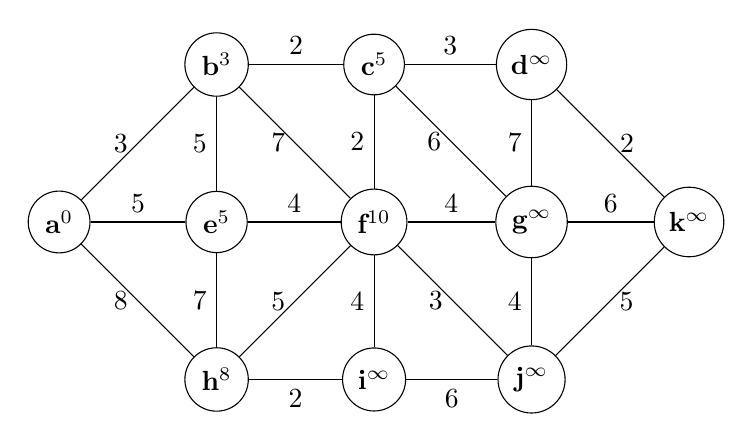
\begin{tikzpicture}
	\node[shape=circle,draw=black] (a) at (0, 2)     {\textbf{a$^0$}};
	\node[shape=circle,draw=black] (b) at (2, 4)     {\textbf{b$^3$}};
	\node[shape=circle,draw=black] (c) at (4, 4)     {\textbf{c$^5$}};
	\node[shape=circle,draw=black] (d) at (6, 4)     {\textbf{d$^\infty$}};
	\node[shape=circle,draw=black] (e) at (2, 2)     {\textbf{e$^5$}};
	\node[shape=circle,draw=black] (f) at (4, 2)     {\textbf{f$^{10}$}};
	\node[shape=circle,draw=black] (g) at (6, 2)     {\textbf{g$^\infty$}};
	\node[shape=circle,draw=black] (h) at (2, 0)     {\textbf{h$^8$}};
	\node[shape=circle,draw=black] (i) at (4, 0)     {\textbf{i$^\infty$}};
	\node[shape=circle,draw=black] (j) at (6, 0)     {\textbf{j$^\infty$}};;
	\node[shape=circle,draw=black] (k) at (8, 2)     {\textbf{k$^\infty$}};

	\path[-] (a) edge node[left]{3} (b);
	\path[-] (a) edge node[above]{5} (e);
	\path[-] (a) edge node[left]{8} (h);
	\path[-] (b) edge node[left]{5} (e);
	\path[-] (b) edge node[left]{7} (f);
	\path[-] (b) edge node[above]{2} (c);
	\path[-] (e) edge node[above]{4} (f);
	\path[-] (e) edge node[left]{7} (h);
	\path[-] (h) edge node[left]{5} (f);	
	\path[-] (h) edge node[below]{2} (i);	
	\path[-] (c) edge node[above]{3} (d);
	\path[-] (c) edge node[left]{6} (g);
	\path[-] (c) edge node[left]{2} (f);
	\path[-] (f) edge node[above]{4} (g);
	\path[-] (f) edge node[left]{3} (j);
	\path[-] (f) edge node[left]{4} (i);
	\path[-] (i) edge node[below]{6} (j);	
	\path[-] (d) edge node[right]{2} (k);
	\path[-] (d) edge node[left]{7} (g);
	\path[-] (g) edge node[above]{6} (k);
	\path[-] (g) edge node[left]{4} (j);
	\path[-] (j) edge node[right]{5} (k);
		
	\end{tikzpicture} 
\caption{The graph after node $b$ has visited}
	\label{gg0}
\end{figure}
The distance costs and routes from node $a$ are as follows;
\begin{itemize}
    \item b: 3 (a)
    \item e: 5 (a)
    \item h: 8 (a)
    \item c: 5 (a,b)
    \item f: 10 (a,b)
\end{itemize}
\textbf{Visited Nodes} : a,b
\subsubsection*{Step 3}
By visiting the \textit{unvisited} neighbouring nodes of $e$, we get the following graph.
\begin{figure}[H]
	\centering
	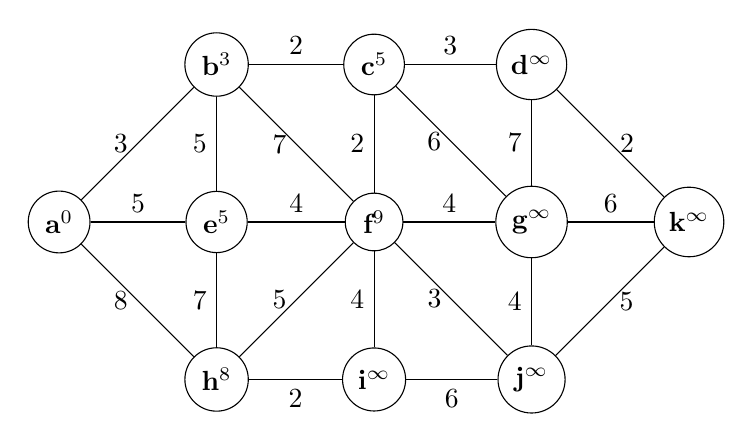
\begin{tikzpicture}
	\node[shape=circle,draw=black] (a) at (0, 2)     {\textbf{a$^0$}};
	\node[shape=circle,draw=black] (b) at (2, 4)     {\textbf{b$^3$}};
	\node[shape=circle,draw=black] (c) at (4, 4)     {\textbf{c$^5$}};
	\node[shape=circle,draw=black] (d) at (6, 4)     {\textbf{d$^\infty$}};
	\node[shape=circle,draw=black] (e) at (2, 2)     {\textbf{e$^5$}};
	\node[shape=circle,draw=black] (f) at (4, 2)     {\textbf{f$^{9}$}};
	\node[shape=circle,draw=black] (g) at (6, 2)     {\textbf{g$^\infty$}};
	\node[shape=circle,draw=black] (h) at (2, 0)     {\textbf{h$^8$}};
	\node[shape=circle,draw=black] (i) at (4, 0)     {\textbf{i$^\infty$}};
	\node[shape=circle,draw=black] (j) at (6, 0)     {\textbf{j$^\infty$}};;
	\node[shape=circle,draw=black] (k) at (8, 2)     {\textbf{k$^\infty$}};

	\path[-] (a) edge node[left]{3} (b);
	\path[-] (a) edge node[above]{5} (e);
	\path[-] (a) edge node[left]{8} (h);
	\path[-] (b) edge node[left]{5} (e);
	\path[-] (b) edge node[left]{7} (f);
	\path[-] (b) edge node[above]{2} (c);
	\path[-] (e) edge node[above]{4} (f);
	\path[-] (e) edge node[left]{7} (h);
	\path[-] (h) edge node[left]{5} (f);	
	\path[-] (h) edge node[below]{2} (i);	
	\path[-] (c) edge node[above]{3} (d);
	\path[-] (c) edge node[left]{6} (g);
	\path[-] (c) edge node[left]{2} (f);
	\path[-] (f) edge node[above]{4} (g);
	\path[-] (f) edge node[left]{3} (j);
	\path[-] (f) edge node[left]{4} (i);
	\path[-] (i) edge node[below]{6} (j);	
	\path[-] (d) edge node[right]{2} (k);
	\path[-] (d) edge node[left]{7} (g);
	\path[-] (g) edge node[above]{6} (k);
	\path[-] (g) edge node[left]{4} (j);
	\path[-] (j) edge node[right]{5} (k);
		
	\end{tikzpicture} 
\caption{The graph after node $e$ has visited}
	\label{gg0}
\end{figure}
The distance costs and routes from node $a$ are as follows;
\begin{itemize}
    \item b: 3 (a)
    \item e: 5 (a)
    \item h: 8 (a)
    \item c: 5 (a,b)
    \item f: 9 (a,e)
\end{itemize}
\textbf{Visited Nodes} : a,b,e
\subsubsection*{Step 4}
By visiting the \textit{unvisited} neighbouring nodes of $h$, we get the following graph.
\begin{figure}[H]
	\centering
	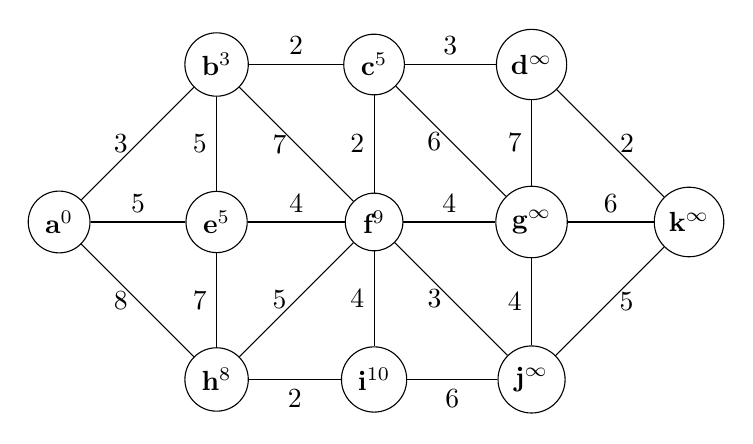
\begin{tikzpicture}
	\node[shape=circle,draw=black] (a) at (0, 2)     {\textbf{a$^0$}};
	\node[shape=circle,draw=black] (b) at (2, 4)     {\textbf{b$^3$}};
	\node[shape=circle,draw=black] (c) at (4, 4)     {\textbf{c$^5$}};
	\node[shape=circle,draw=black] (d) at (6, 4)     {\textbf{d$^\infty$}};
	\node[shape=circle,draw=black] (e) at (2, 2)     {\textbf{e$^5$}};
	\node[shape=circle,draw=black] (f) at (4, 2)     {\textbf{f$^{9}$}};
	\node[shape=circle,draw=black] (g) at (6, 2)     {\textbf{g$^\infty$}};
	\node[shape=circle,draw=black] (h) at (2, 0)     {\textbf{h$^8$}};
	\node[shape=circle,draw=black] (i) at (4, 0)     {\textbf{i$^{10}$}};
	\node[shape=circle,draw=black] (j) at (6, 0)     {\textbf{j$^\infty$}};;
	\node[shape=circle,draw=black] (k) at (8, 2)     {\textbf{k$^\infty$}};

	\path[-] (a) edge node[left]{3} (b);
	\path[-] (a) edge node[above]{5} (e);
	\path[-] (a) edge node[left]{8} (h);
	\path[-] (b) edge node[left]{5} (e);
	\path[-] (b) edge node[left]{7} (f);
	\path[-] (b) edge node[above]{2} (c);
	\path[-] (e) edge node[above]{4} (f);
	\path[-] (e) edge node[left]{7} (h);
	\path[-] (h) edge node[left]{5} (f);	
	\path[-] (h) edge node[below]{2} (i);	
	\path[-] (c) edge node[above]{3} (d);
	\path[-] (c) edge node[left]{6} (g);
	\path[-] (c) edge node[left]{2} (f);
	\path[-] (f) edge node[above]{4} (g);
	\path[-] (f) edge node[left]{3} (j);
	\path[-] (f) edge node[left]{4} (i);
	\path[-] (i) edge node[below]{6} (j);	
	\path[-] (d) edge node[right]{2} (k);
	\path[-] (d) edge node[left]{7} (g);
	\path[-] (g) edge node[above]{6} (k);
	\path[-] (g) edge node[left]{4} (j);
	\path[-] (j) edge node[right]{5} (k);
		
	\end{tikzpicture} 
\caption{The graph after node $h$ has visited}
	\label{gg0}
\end{figure}
The distance costs and routes from node $a$ are as follows;
\begin{itemize}
    \item b: 3 (a)
    \item e: 5 (a)
    \item h: 8 (a)
    \item c: 5 (a,b)
    \item f: 9 (a,e)
    \item i: 10 (a,h)
\end{itemize}
\textbf{Visited Nodes} : a,b,e,h
\subsubsection*{Step 5}
By visiting the \textit{unvisited} neighbouring nodes of $c$, we get the following graph.
\begin{figure}[H]
	\centering
	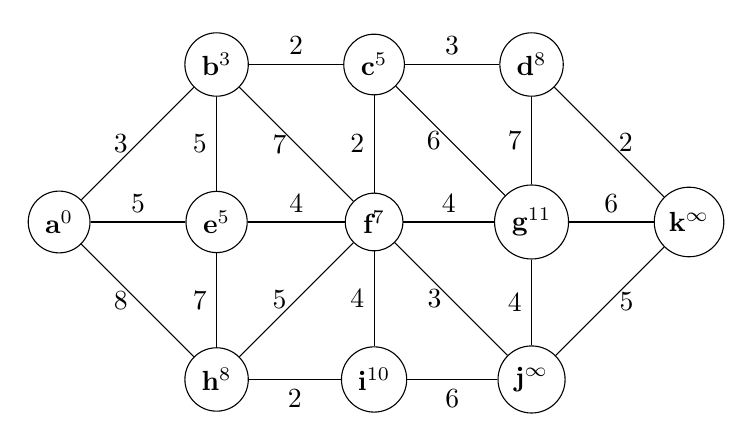
\begin{tikzpicture}
	\node[shape=circle,draw=black] (a) at (0, 2)     {\textbf{a$^0$}};
	\node[shape=circle,draw=black] (b) at (2, 4)     {\textbf{b$^3$}};
	\node[shape=circle,draw=black] (c) at (4, 4)     {\textbf{c$^5$}};
	\node[shape=circle,draw=black] (d) at (6, 4)     {\textbf{d$^8$}};
	\node[shape=circle,draw=black] (e) at (2, 2)     {\textbf{e$^5$}};
	\node[shape=circle,draw=black] (f) at (4, 2)     {\textbf{f$^{7}$}};
	\node[shape=circle,draw=black] (g) at (6, 2)     {\textbf{g$^{11}$}};
	\node[shape=circle,draw=black] (h) at (2, 0)     {\textbf{h$^8$}};
	\node[shape=circle,draw=black] (i) at (4, 0)     {\textbf{i$^{10}$}};
	\node[shape=circle,draw=black] (j) at (6, 0)     {\textbf{j$^\infty$}};;
	\node[shape=circle,draw=black] (k) at (8, 2)     {\textbf{k$^\infty$}};

	\path[-] (a) edge node[left]{3} (b);
	\path[-] (a) edge node[above]{5} (e);
	\path[-] (a) edge node[left]{8} (h);
	\path[-] (b) edge node[left]{5} (e);
	\path[-] (b) edge node[left]{7} (f);
	\path[-] (b) edge node[above]{2} (c);
	\path[-] (e) edge node[above]{4} (f);
	\path[-] (e) edge node[left]{7} (h);
	\path[-] (h) edge node[left]{5} (f);	
	\path[-] (h) edge node[below]{2} (i);	
	\path[-] (c) edge node[above]{3} (d);
	\path[-] (c) edge node[left]{6} (g);
	\path[-] (c) edge node[left]{2} (f);
	\path[-] (f) edge node[above]{4} (g);
	\path[-] (f) edge node[left]{3} (j);
	\path[-] (f) edge node[left]{4} (i);
	\path[-] (i) edge node[below]{6} (j);	
	\path[-] (d) edge node[right]{2} (k);
	\path[-] (d) edge node[left]{7} (g);
	\path[-] (g) edge node[above]{6} (k);
	\path[-] (g) edge node[left]{4} (j);
	\path[-] (j) edge node[right]{5} (k);
		
	\end{tikzpicture} 
\caption{The graph after node $c$ has visited}
	\label{gg0}
\end{figure}
The distance costs and routes from node $a$ are as follows;
\begin{itemize}
    \item b: 3 (a)
    \item e: 5 (a)
    \item h: 8 (a)
    \item c: 5 (a,b)
    \item f: 7 (a,b,c)
    \item i: 10 (a,h)
    \item d: 8 (a,b,c)
    \item g: 11 (a,b,c)
\end{itemize}
\textbf{Visited Nodes} : a,b,e,h,c
\subsubsection*{Step 6}
By visiting the \textit{unvisited} neighbouring nodes of $f$, we get the following graph.
\begin{figure}[H]
	\centering
	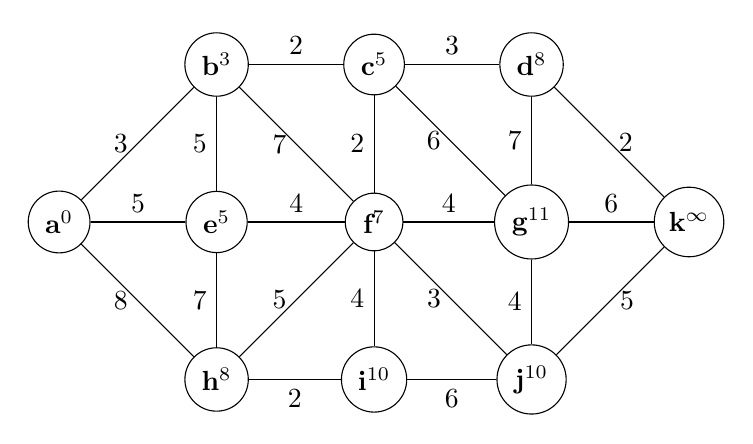
\begin{tikzpicture}
	\node[shape=circle,draw=black] (a) at (0, 2)     {\textbf{a$^0$}};
	\node[shape=circle,draw=black] (b) at (2, 4)     {\textbf{b$^3$}};
	\node[shape=circle,draw=black] (c) at (4, 4)     {\textbf{c$^5$}};
	\node[shape=circle,draw=black] (d) at (6, 4)     {\textbf{d$^8$}};
	\node[shape=circle,draw=black] (e) at (2, 2)     {\textbf{e$^5$}};
	\node[shape=circle,draw=black] (f) at (4, 2)     {\textbf{f$^{7}$}};
	\node[shape=circle,draw=black] (g) at (6, 2)     {\textbf{g$^{11}$}};
	\node[shape=circle,draw=black] (h) at (2, 0)     {\textbf{h$^8$}};
	\node[shape=circle,draw=black] (i) at (4, 0)     {\textbf{i$^{10}$}};
	\node[shape=circle,draw=black] (j) at (6, 0)     {\textbf{j$^{10}$}};;
	\node[shape=circle,draw=black] (k) at (8, 2)     {\textbf{k$^\infty$}};

	\path[-] (a) edge node[left]{3} (b);
	\path[-] (a) edge node[above]{5} (e);
	\path[-] (a) edge node[left]{8} (h);
	\path[-] (b) edge node[left]{5} (e);
	\path[-] (b) edge node[left]{7} (f);
	\path[-] (b) edge node[above]{2} (c);
	\path[-] (e) edge node[above]{4} (f);
	\path[-] (e) edge node[left]{7} (h);
	\path[-] (h) edge node[left]{5} (f);	
	\path[-] (h) edge node[below]{2} (i);	
	\path[-] (c) edge node[above]{3} (d);
	\path[-] (c) edge node[left]{6} (g);
	\path[-] (c) edge node[left]{2} (f);
	\path[-] (f) edge node[above]{4} (g);
	\path[-] (f) edge node[left]{3} (j);
	\path[-] (f) edge node[left]{4} (i);
	\path[-] (i) edge node[below]{6} (j);	
	\path[-] (d) edge node[right]{2} (k);
	\path[-] (d) edge node[left]{7} (g);
	\path[-] (g) edge node[above]{6} (k);
	\path[-] (g) edge node[left]{4} (j);
	\path[-] (j) edge node[right]{5} (k);
		
	\end{tikzpicture} 
\caption{The graph after node $f$ has visited}
	\label{gg0}
\end{figure}
The distance costs and routes from node $a$ are as follows;
\begin{itemize}
    \item b: 3 (a)
    \item e: 5 (a)
    \item h: 8 (a)
    \item c: 5 (a,b)
    \item f: 7 (a,b,c)
    \item i: 10 (a,h)
    \item d: 8 (a,b,c)
    \item g: 11 (a,b,c)
    \item j: 10 (a,b,c,f)
\end{itemize}
\textbf{Visited Nodes} : a,b,e,h,c,f
\subsubsection*{Step 7}
By visiting the \textit{unvisited} neighbouring nodes of $i$, we get the following graph.
\begin{figure}[H]
	\centering
	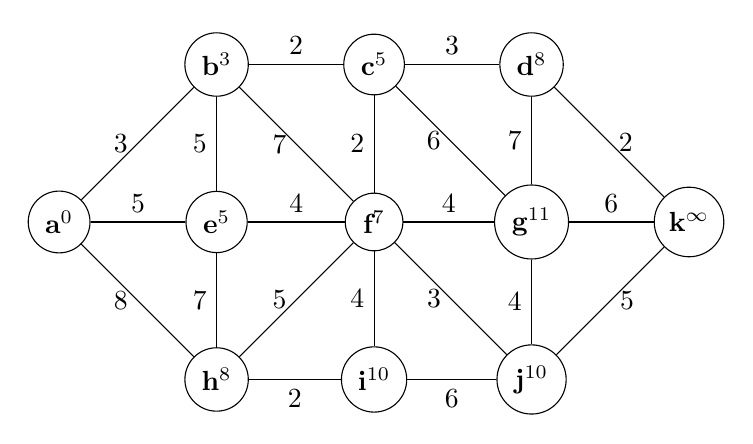
\begin{tikzpicture}
	\node[shape=circle,draw=black] (a) at (0, 2)     {\textbf{a$^0$}};
	\node[shape=circle,draw=black] (b) at (2, 4)     {\textbf{b$^3$}};
	\node[shape=circle,draw=black] (c) at (4, 4)     {\textbf{c$^5$}};
	\node[shape=circle,draw=black] (d) at (6, 4)     {\textbf{d$^8$}};
	\node[shape=circle,draw=black] (e) at (2, 2)     {\textbf{e$^5$}};
	\node[shape=circle,draw=black] (f) at (4, 2)     {\textbf{f$^{7}$}};
	\node[shape=circle,draw=black] (g) at (6, 2)     {\textbf{g$^{11}$}};
	\node[shape=circle,draw=black] (h) at (2, 0)     {\textbf{h$^8$}};
	\node[shape=circle,draw=black] (i) at (4, 0)     {\textbf{i$^{10}$}};
	\node[shape=circle,draw=black] (j) at (6, 0)     {\textbf{j$^{10}$}};;
	\node[shape=circle,draw=black] (k) at (8, 2)     {\textbf{k$^\infty$}};

	\path[-] (a) edge node[left]{3} (b);
	\path[-] (a) edge node[above]{5} (e);
	\path[-] (a) edge node[left]{8} (h);
	\path[-] (b) edge node[left]{5} (e);
	\path[-] (b) edge node[left]{7} (f);
	\path[-] (b) edge node[above]{2} (c);
	\path[-] (e) edge node[above]{4} (f);
	\path[-] (e) edge node[left]{7} (h);
	\path[-] (h) edge node[left]{5} (f);	
	\path[-] (h) edge node[below]{2} (i);	
	\path[-] (c) edge node[above]{3} (d);
	\path[-] (c) edge node[left]{6} (g);
	\path[-] (c) edge node[left]{2} (f);
	\path[-] (f) edge node[above]{4} (g);
	\path[-] (f) edge node[left]{3} (j);
	\path[-] (f) edge node[left]{4} (i);
	\path[-] (i) edge node[below]{6} (j);	
	\path[-] (d) edge node[right]{2} (k);
	\path[-] (d) edge node[left]{7} (g);
	\path[-] (g) edge node[above]{6} (k);
	\path[-] (g) edge node[left]{4} (j);
	\path[-] (j) edge node[right]{5} (k);
		
	\end{tikzpicture} 
\caption{The graph after node $i$ has visited}
	\label{gg0}
\end{figure}
The distance costs and routes from node $a$ are as follows;
\begin{itemize}
    \item b: 3 (a)
    \item e: 5 (a)
    \item h: 8 (a)
    \item c: 5 (a,b)
    \item f: 7 (a,b,c)
    \item i: 10 (a,h)
    \item d: 8 (a,b,c)
    \item g: 11 (a,b,c)
    \item j: 10 (a,b,c,f)
\end{itemize}
\textbf{Visited Nodes} : a,b,e,h,c,f,i
\subsubsection*{Step 8}
By visiting the \textit{unvisited} neighbouring nodes of $d$, we get the following graph.
\begin{figure}[H]
	\centering
	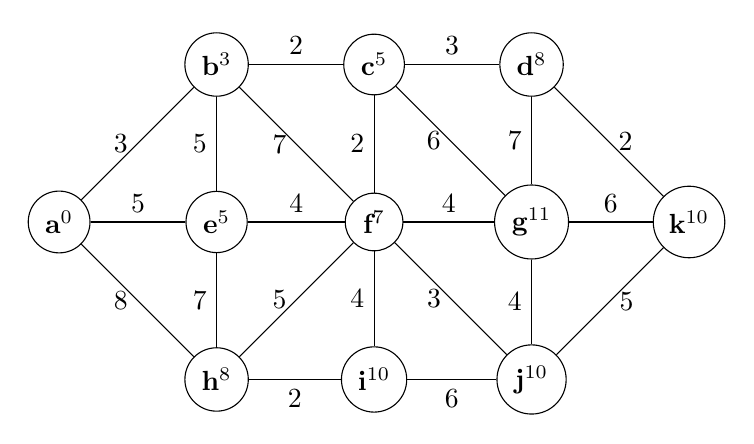
\begin{tikzpicture}
	\node[shape=circle,draw=black] (a) at (0, 2)     {\textbf{a$^0$}};
	\node[shape=circle,draw=black] (b) at (2, 4)     {\textbf{b$^3$}};
	\node[shape=circle,draw=black] (c) at (4, 4)     {\textbf{c$^5$}};
	\node[shape=circle,draw=black] (d) at (6, 4)     {\textbf{d$^8$}};
	\node[shape=circle,draw=black] (e) at (2, 2)     {\textbf{e$^5$}};
	\node[shape=circle,draw=black] (f) at (4, 2)     {\textbf{f$^{7}$}};
	\node[shape=circle,draw=black] (g) at (6, 2)     {\textbf{g$^{11}$}};
	\node[shape=circle,draw=black] (h) at (2, 0)     {\textbf{h$^8$}};
	\node[shape=circle,draw=black] (i) at (4, 0)     {\textbf{i$^{10}$}};
	\node[shape=circle,draw=black] (j) at (6, 0)     {\textbf{j$^{10}$}};;
	\node[shape=circle,draw=black] (k) at (8, 2)     {\textbf{k$^{10}$}};

	\path[-] (a) edge node[left]{3} (b);
	\path[-] (a) edge node[above]{5} (e);
	\path[-] (a) edge node[left]{8} (h);
	\path[-] (b) edge node[left]{5} (e);
	\path[-] (b) edge node[left]{7} (f);
	\path[-] (b) edge node[above]{2} (c);
	\path[-] (e) edge node[above]{4} (f);
	\path[-] (e) edge node[left]{7} (h);
	\path[-] (h) edge node[left]{5} (f);	
	\path[-] (h) edge node[below]{2} (i);	
	\path[-] (c) edge node[above]{3} (d);
	\path[-] (c) edge node[left]{6} (g);
	\path[-] (c) edge node[left]{2} (f);
	\path[-] (f) edge node[above]{4} (g);
	\path[-] (f) edge node[left]{3} (j);
	\path[-] (f) edge node[left]{4} (i);
	\path[-] (i) edge node[below]{6} (j);	
	\path[-] (d) edge node[right]{2} (k);
	\path[-] (d) edge node[left]{7} (g);
	\path[-] (g) edge node[above]{6} (k);
	\path[-] (g) edge node[left]{4} (j);
	\path[-] (j) edge node[right]{5} (k);
		
	\end{tikzpicture} 
\caption{The graph after node $d$ has visited}
	\label{gg0}
\end{figure}
The distance costs and routes from node $a$ are as follows;
\begin{itemize}
    \item b: 3 (a)
    \item e: 5 (a)
    \item h: 8 (a)
    \item c: 5 (a,b)
    \item f: 7 (a,b,c)
    \item i: 10 (a,h)
    \item d: 8 (a,b,c)
    \item g: 11 (a,b,c)
    \item j: 10 (a,b,c,f)
    \item k: 10 (a,b,c,d)
\end{itemize}
\textbf{Visited Nodes} : a,b,e,h,c,f,i,d
\subsubsection*{Step 9}
By visiting the \textit{unvisited} neighbouring nodes of $j$, we get the following graph.
\begin{figure}[H]
	\centering
	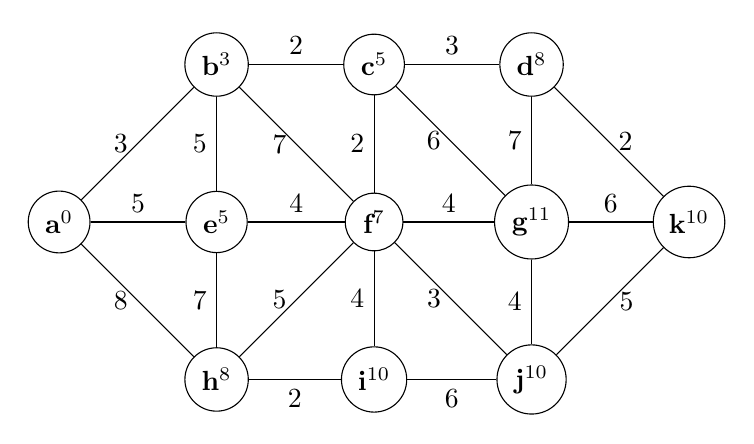
\begin{tikzpicture}
	\node[shape=circle,draw=black] (a) at (0, 2)     {\textbf{a$^0$}};
	\node[shape=circle,draw=black] (b) at (2, 4)     {\textbf{b$^3$}};
	\node[shape=circle,draw=black] (c) at (4, 4)     {\textbf{c$^5$}};
	\node[shape=circle,draw=black] (d) at (6, 4)     {\textbf{d$^8$}};
	\node[shape=circle,draw=black] (e) at (2, 2)     {\textbf{e$^5$}};
	\node[shape=circle,draw=black] (f) at (4, 2)     {\textbf{f$^{7}$}};
	\node[shape=circle,draw=black] (g) at (6, 2)     {\textbf{g$^{11}$}};
	\node[shape=circle,draw=black] (h) at (2, 0)     {\textbf{h$^8$}};
	\node[shape=circle,draw=black] (i) at (4, 0)     {\textbf{i$^{10}$}};
	\node[shape=circle,draw=black] (j) at (6, 0)     {\textbf{j$^{10}$}};;
	\node[shape=circle,draw=black] (k) at (8, 2)     {\textbf{k$^{10}$}};

	\path[-] (a) edge node[left]{3} (b);
	\path[-] (a) edge node[above]{5} (e);
	\path[-] (a) edge node[left]{8} (h);
	\path[-] (b) edge node[left]{5} (e);
	\path[-] (b) edge node[left]{7} (f);
	\path[-] (b) edge node[above]{2} (c);
	\path[-] (e) edge node[above]{4} (f);
	\path[-] (e) edge node[left]{7} (h);
	\path[-] (h) edge node[left]{5} (f);	
	\path[-] (h) edge node[below]{2} (i);	
	\path[-] (c) edge node[above]{3} (d);
	\path[-] (c) edge node[left]{6} (g);
	\path[-] (c) edge node[left]{2} (f);
	\path[-] (f) edge node[above]{4} (g);
	\path[-] (f) edge node[left]{3} (j);
	\path[-] (f) edge node[left]{4} (i);
	\path[-] (i) edge node[below]{6} (j);	
	\path[-] (d) edge node[right]{2} (k);
	\path[-] (d) edge node[left]{7} (g);
	\path[-] (g) edge node[above]{6} (k);
	\path[-] (g) edge node[left]{4} (j);
	\path[-] (j) edge node[right]{5} (k);
		
	\end{tikzpicture} 
\caption{The graph after node $j$ has visited}
	\label{gg0}
\end{figure}
The distance costs and routes from node $a$ are as follows;
\begin{itemize}
    \item b: 3 (a)
    \item e: 5 (a)
    \item h: 8 (a)
    \item c: 5 (a,b)
    \item f: 7 (a,b,c)
    \item i: 10 (a,h)
    \item d: 8 (a,b,c)
    \item g: 11 (a,b,c)
    \item j: 10 (a,b,c,f)
    \item k: 10 (a,b,c,d)
\end{itemize}
\textbf{Visited Nodes} : a,b,e,h,c,f,i,d,j
\subsubsection*{Step 10}
By visiting the \textit{unvisited} neighbouring nodes of $d$, we get the following graph.
\begin{figure}[H]
	\centering
	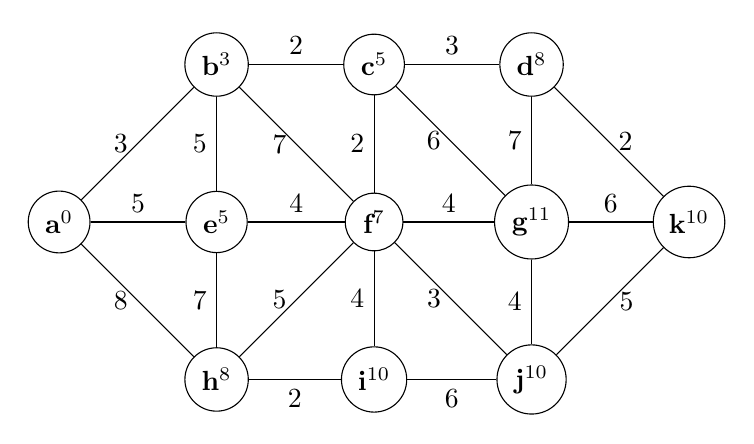
\begin{tikzpicture}
	\node[shape=circle,draw=black] (a) at (0, 2)     {\textbf{a$^0$}};
	\node[shape=circle,draw=black] (b) at (2, 4)     {\textbf{b$^3$}};
	\node[shape=circle,draw=black] (c) at (4, 4)     {\textbf{c$^5$}};
	\node[shape=circle,draw=black] (d) at (6, 4)     {\textbf{d$^8$}};
	\node[shape=circle,draw=black] (e) at (2, 2)     {\textbf{e$^5$}};
	\node[shape=circle,draw=black] (f) at (4, 2)     {\textbf{f$^{7}$}};
	\node[shape=circle,draw=black] (g) at (6, 2)     {\textbf{g$^{11}$}};
	\node[shape=circle,draw=black] (h) at (2, 0)     {\textbf{h$^8$}};
	\node[shape=circle,draw=black] (i) at (4, 0)     {\textbf{i$^{10}$}};
	\node[shape=circle,draw=black] (j) at (6, 0)     {\textbf{j$^{10}$}};;
	\node[shape=circle,draw=black] (k) at (8, 2)     {\textbf{k$^{10}$}};

	\path[-] (a) edge node[left]{3} (b);
	\path[-] (a) edge node[above]{5} (e);
	\path[-] (a) edge node[left]{8} (h);
	\path[-] (b) edge node[left]{5} (e);
	\path[-] (b) edge node[left]{7} (f);
	\path[-] (b) edge node[above]{2} (c);
	\path[-] (e) edge node[above]{4} (f);
	\path[-] (e) edge node[left]{7} (h);
	\path[-] (h) edge node[left]{5} (f);	
	\path[-] (h) edge node[below]{2} (i);	
	\path[-] (c) edge node[above]{3} (d);
	\path[-] (c) edge node[left]{6} (g);
	\path[-] (c) edge node[left]{2} (f);
	\path[-] (f) edge node[above]{4} (g);
	\path[-] (f) edge node[left]{3} (j);
	\path[-] (f) edge node[left]{4} (i);
	\path[-] (i) edge node[below]{6} (j);	
	\path[-] (d) edge node[right]{2} (k);
	\path[-] (d) edge node[left]{7} (g);
	\path[-] (g) edge node[above]{6} (k);
	\path[-] (g) edge node[left]{4} (j);
	\path[-] (j) edge node[right]{5} (k);
		
	\end{tikzpicture} 
\caption{The graph after node $d$ has visited}
	\label{gg0}
\end{figure}
The distance costs and routes from node $a$ are as follows;
\begin{itemize}
    \item b: 3 (a)
    \item e: 5 (a)
    \item h: 8 (a)
    \item c: 5 (a,b)
    \item f: 7 (a,b,c)
    \item i: 10 (a,h)
    \item d: 8 (a,b,c)
    \item g: 11 (a,b,c)
    \item j: 10 (a,b,c,f)
    \item k: 10 (a,b,c,d)
\end{itemize}
\textbf{Visited Nodes} : a,b,e,h,c,f,i,d,j,g
\subsubsection*{Step 11}
Since there are no \textit{unvisited} neighbouring nodes of $j$, we concluded our traversal. \\
The shortest path from $a$ to $j$ by using \textbf{Dijkstra's Algorithm} is: $ a \rightarrow b \rightarrow c \rightarrow f \rightarrow j$, and it has a distance cost of $10$.
\subsection*{b)}
By following the choices below, 
\begin{table}[H]
    \centering
    \renewcommand{\arraystretch}{1.25}
    \begin{tabular}{|c|c|c|p{114mm}|}	
    \hline 							
   \textbf{Choice} & \textbf{Edge} & \textbf{Weight} & \textbf{Reason} \\
    \hline 
    \hline 
    1 & [a,b] & 3 & From the vertex $a$, we start with picking the smallest weighted edge. \\ \hline
    2 & [b,c] & 2 & From the vertices $a$ and $b$, the smallest weighted edge is $b-c$, with a weight of 2. \\ \hline
    3 & [c,f] & 2 & From the vertices $a$, $b$ and $c$, the smallest weighted edge is $c-f$, with a weight of 2.\\ \hline
    4 & [c,d] & 3 & From the vertices  $a$, $b$,$c$, and $f$, the smallest weighted edge is $c-d$, with a weight of 3.\\ \hline
    5 & [d,k] & 2 & From the vertices $a$, $b$, $c$, $d$ and $f$, the smallest weighted edge is $d-k$, with a weight of 2. \\ \hline
    6 & [f,j] & 3 & From the vertices $a$, $b$, $c$, $f$, $d$ and $k$, the smallest weighted edge is $f-j$, with weights of 3.\\ \hline
    7 & [f,i] & 4 & From the vertices $a$, $b$, $c$, $f$, $d$, $k$ and $j$, the smallest weighted edges are $f-i$ and $f-e$, and $f-g$, with a weight of 4.  We can choose any of them, and we proceed with $f-i$.\\ \hline
    8 & [i,h] & 2 & From the vertices $a$, $b$, $c$, $f$, $d$, $k$, $i$ and $j$, the smallest weighted edge is $i-h$, with weight of 2. \\ \hline
    9 & [f,e] & 4 & From the vertices $a$, $b$, $c$, $f$, $d$, $k$,$h$, $i$ and $j$, the smallest weighted edges are $f-e$ and $j-g$, and $f-g$, with a weight of 4. We can choose any of them, and we proceed with $f-e$.\\ \hline
    10 & [j,g] & 4 & From the vertices $a$, $b$, $c$, $f$, $d$, $k$,$h$, $i$ and $j$, the smallest weighted edges are $j-g$ and $f-g$ with a weight of 4. We can choose any of them, and we proceed with $j-g$. \\ \hline        
    \end{tabular}
    \caption{ Procedure of creating a minimum spanning tree of Graph G in Q5 produced using Prim's Algorithm }
    \end{table}
    
We conclude the minimum spanning tree, since picking any of the remaining edges would form \textit{simple circuits}. \\

The minimum spanning tree of the graph can be seen below(the used edges to find the minimum spanning tree, are denoted with a \textit{thicker} edge).
\begin{figure}[H]
	\centering
	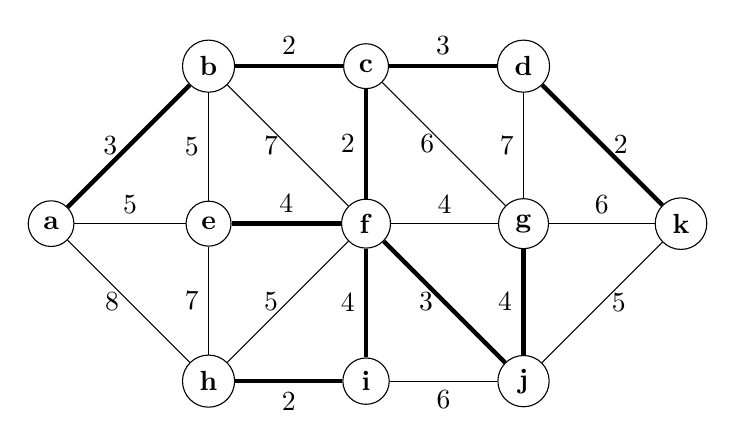
\begin{tikzpicture}
	\node[shape=circle,draw=black] (a) at (0, 2)     {\textbf{a}};
	\node[shape=circle,draw=black] (b) at (2, 4)     {\textbf{b}};
	\node[shape=circle,draw=black] (c) at (4, 4)     {\textbf{c}};
	\node[shape=circle,draw=black] (d) at (6, 4)     {\textbf{d}};
	\node[shape=circle,draw=black] (e) at (2, 2)     {\textbf{e}};
	\node[shape=circle,draw=black] (f) at (4, 2)     {\textbf{f}};
	\node[shape=circle,draw=black] (g) at (6, 2)     {\textbf{g}};
	\node[shape=circle,draw=black] (h) at (2, 0)     {\textbf{h}};
	\node[shape=circle,draw=black] (i) at (4, 0)     {\textbf{i}};
	\node[shape=circle,draw=black] (j) at (6, 0)     {\textbf{j}};
	\node[shape=circle,draw=black] (k) at (8, 2)     {\textbf{k}};

	\path[-][ultra thick] (a) edge node[left]{3} (b);
	\path[-] (a) edge node[above]{5} (e);
	\path[-] (a) edge node[left]{8} (h);
	\path[-] (b) edge node[left]{5} (e);
	\path[-] (b) edge node[left]{7} (f);
	\path[-][ultra thick] (b) edge node[above]{2} (c);
	\path[-][ultra thick] (e) edge node[above]{4} (f);
	\path[-] (e) edge node[left]{7} (h);
	\path[-] (h) edge node[left]{5} (f);	
	\path[-][ultra thick] (h) edge node[below]{2} (i);	
	\path[-][ultra thick] (c) edge node[above]{3} (d);
	\path[-] (c) edge node[left]{6} (g);
	\path[-][ultra thick] (c) edge node[left]{2} (f);
	\path[-] (f) edge node[above]{4} (g);
	\path[-][ultra thick] (f) edge node[left]{3} (j);
	\path[-][ultra thick] (f) edge node[left]{4} (i);
	\path[-] (i) edge node[below]{6} (j);	
	\path[-][ultra thick] (d) edge node[right]{2} (k);
	\path[-] (d) edge node[left]{7} (g);
	\path[-] (g) edge node[above]{6} (k);
	\path[-][ultra thick] (g) edge node[left]{4} (j);
	\path[-] (j) edge node[right]{5} (k);
		
	\end{tikzpicture} 
	\caption{A minimum spanning tree of Graph G in Q5 produced using Prim's Algorithm}
	\label{g5}
\end{figure}
\pagebreak
\section*{Answer 6}
\subsection*{a)}
There are \textbf{7} vertices, \textbf{6} edges on $T$, and it has a height of \textbf{3}.
\subsection*{b)}
\texttt{<a:17>,<b:13>,<c:24>,<d:19>,<e:43>,<f:23>,<g:58>}
\subsection*{c)}
\texttt{<b:13>,<d:19>,<f:23>,<g:58>,<e:43>,<c:24>,<a:17>}
\subsection*{d)}
\texttt{<b:13>,<a:17>,<d:19>,<c:24>,<f:23>,<e:43>,<g:58>}
\subsection*{e)}
\begin{itemize}
    \item
    \begin{quote}
        The tree is called a \textit{full m-ary tree} if every internal vertex has exactly $m$ children. An \textit{m-ary} tree with $m$ = 2 is called a binary tree.(Definition 3, pg.784)
    \end{quote}
    \item When we look at $T$, we can see that \texttt{<a:17>,<c:24>,and <e:43>} have 2 children each. Therefore $T$ is a full binary tree.
\end{itemize}    
\subsection*{f)}
T is a full binary tree however, not all the leaves are at the same level. From that, T is not a complete binary tree.\\
\subsection*{g)}
\begin{itemize}
    \item On a Binary Search Tree, if we do a Inorder Traversal,  since the inorder traversal would follow left-root-right order, and since the left child will always be smaller than the root, similarly the right child will always be greater than the root; we should get ordered keys as the output.
    \item When we take a look at the inorder traversal of $T$, we can see that the pair \texttt{<c:24>,<f:23>} is not sorted properly. 
    \item Therefore we can easily say that the given tree $T$ is not a binary search tree.
\end{itemize}

\subsection*{h)}
One can see that by developing a recursive definition, n$_h$ =  n$_{h-1}$ + 2; with initial condition n$_0$ = 1.\\
Where h is the height and n$_h$ is the minimum number of nodes for a full binary tree with height \textit{h} \\
n$_{5}$ =\textbf{11}\\
\subsection*{i)}
\begin{figure}[H]
	\centering
	\begin{tikzpicture}
	
	\node[shape=circle,draw=black] (a) at (6, 8)     {\textbf{4}};
	\node[shape=circle,draw=black] (b) at (3, 6)     {\textbf{2}};
	\node[shape=circle,draw=black] (c) at (9.2, 6)     {\textbf{6}};
	
	\node[shape=circle,draw=black] (d) at (1, 4)     {\textbf{1}};
	\node[shape=circle,draw=black] (e) at (5, 4)     {\textbf{3}};
	\node[shape=circle,draw=black] (f) at (7, 4)     {\textbf{5}};

		
	\path[-] (a) edge (b);
	\path[-] (c) edge (a);
    \path[-] (b) edge (d);
    \path[-] (b) edge (e);
    \path[-] (c) edge (f);
	\end{tikzpicture} 
	\caption{Binary Search Tree by using the integer keys \{1,2,3,4,5,6\}, employing the $\leq$ relation defined on \textbf{Z}*\textbf{Z}}	
	\label{bintreeq6}
\end{figure}

\subsection*{j)}
\begin{itemize}
    \item Sequence to find 1: \texttt{4} $\xrightarrow{\text{left}}$ \texttt{2} $\xrightarrow{\text{left}}$ \texttt{1} 
    \item Sequence to find 6: \texttt{4} $\xrightarrow{\text{right}}$ \texttt{6} 
    
\end{itemize}
\subsection*{k)}
\begin{figure}[H]
	\centering
	\begin{tikzpicture}
	
	\node[shape=circle,draw=black] (g) at (6, 10)     {\textbf{g}};
	
	\node[shape=circle,draw=black] (d) at (6, 8)     {\textbf{d}};
	
	\node[shape=circle,draw=black] (e) at (3, 6)     {\textbf{e}};
	\node[shape=circle,draw=black] (c) at (6, 6)     {\textbf{c}};
	\node[shape=circle,draw=black] (a) at (9, 6)     {\textbf{a}};
	
	\node[shape=circle,draw=black] (f) at (3, 4)     {\textbf{f}};
	
	\node[shape=circle,draw=black] (b) at (3, 2)     {\textbf{b}};

		
	\path[-] (g) edge (d);
	\path[-] (d) edge (e);
    \path[-] (d) edge (c);
    \path[-] (d) edge (a);
    \path[-] (e) edge (f);
    \path[-] (b) edge (f);
	\end{tikzpicture} 
	\caption{Spanning tree for the directed graph G in Q1 via 'Breadth-first Search' }	
	\label{bintreeq6}
\end{figure}
\subsection*{l)}
One can see that by developing a recursive definition, h$_k$ =  h$_{k-1}$ + 1; with initial condition h$_1$ = 0.\\
Where k is the number of vertices in binary search tree and h$_k$ is the maximum height to create a binary search tree containing k vertices. Therefore, h$_k$ =  h$_{k-1}$ + 1 \\
\end{document}

​


